
\chapter{Simulation Code}
\label{ch:simCode}

The full code repository for the particle identification software and fast ARICH simulation is available at \url{https://github.com/danielTLevy/ARICHSim}.

To install, run the following procedure:

\begin{enumerate}
\item Clone repository from GitHub/
\item Ensure ROOT version 6 is installed.
\item Source ROOT from the directory in which it is installed: \\ \verb!source [root_install_dir]/bin/thisroot.sh!
\item run \verb!make! in the \verb!ARICHSim! directory. This will create the executable file \verb!arichsim!.
\end{enumerate}

A UML class diagram demonstrating the main classes and methods in the software is shown in Figure \ref{fig:uml}. 
The software takes in as input a \verb!.root! file containing a 2-dimensional histogram (represented in ROOT as a \verb!TH2D! object) containing information about the $x$ and $y$ positions on the detector plane of each detected photon hit in an event.
It also takes in as arguments a set of positions, directions, and momenta to be used for the simulation.

These arguments gets passed into the \verb!identifyParticle()! method, contained in the file \verb!analysis.cpp!.
This method uses the position and direction parameters to create an instance of the \verb!Arich! class, which is described in \verb!arich.cpp!, and controls the fast simulation of particles passing through the ARICH detector.
The \verb!identifyParticle()! method takes in the given momentum parameter, and calculates particle velocities for each candidate particle to be investigated.
Each velocity then gets passed into the \verb!Arich! instance, which calculates a photon distribution function for the given particle initial position, direction, and velocity, and returns it in the form of a \verb!TH2D!.
Each of the returned photon distributions gets compared to the original event \verb!TH2D! and a negative log-likelihood is computed.
The simulation then reports the negative log-likelihoods, and returns the particle hypothesis that would return the minimum value.

The \verb!Arich! class contains instances of the  \verb!Beam! and  \verb!Detector! classes, and two instances of the  \verb!Aerogel! class, representing the two layers of aerogel.
The  \verb!Beam! class generates a pre-specified number of \verb!Particle! objects, each with a position and direction randomly thrown around the values passed in to the \verb!Arich! class.
Each \verb!Particle! is then passed into the \verb!generatePhotons()! method of both instances of the \verb!Aerogel! class.
This method generates a number of \verb!Photon! objects, each with a position along the given particle's path, a randomly thrown direction, and a randomly thrown wavelength.
The \verb!Arich! class then calls the \verb!scatterPhoton()! method in each \verb!Aerogel! instance, which modifies the direction and position properties of each \verb!Photon! object. 

Each \verb!Photon! object, after having been modified, gets passed to the \verb!Detector! class.
The \verb!Detector! class contains information about the quantum efficiency and geometry of the photon detector plane. 
The \verb!Photon! objects get projected onto this detector, and fills out a \verb!TH2D! object representing the photon distribution of the given particle position, direction, and velocity.

The file \verb!analysis.cpp! contains several scripts to run particle identification on Geant4-generated data, simulate different photon distributions, test particle identification separation, and more. 
Running the \verb!arichsim! executable with no arguments will give a list of possible modes to run in, and will list out the parameters required.


\begin{sidewaysfigure}[]
\centering
\resizebox{1\textwidth}{!}{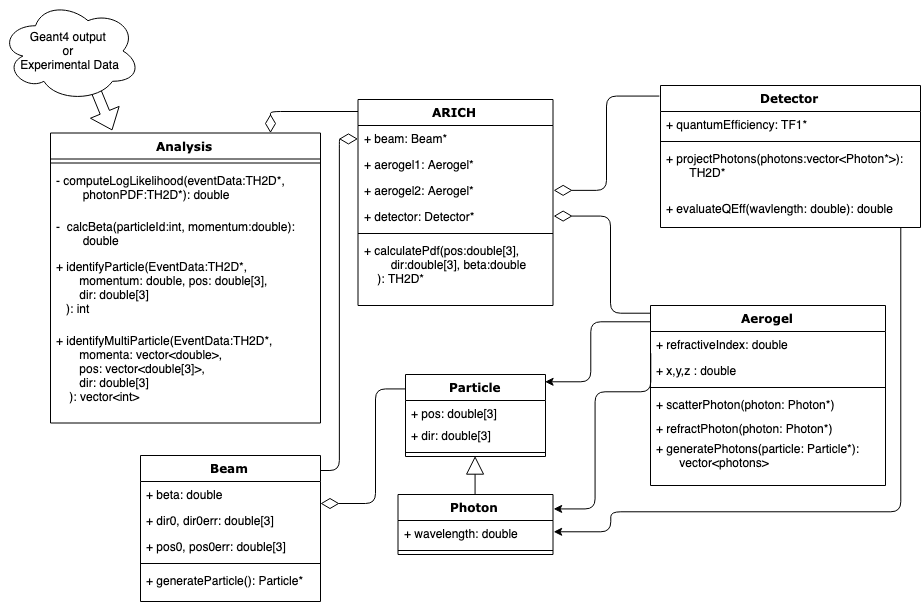
\includegraphics{./figs/uml.png}}
\caption[UML diagram outlining the most important classes and methods used in the simulation and analysis ]{UML diagram outlining the most important classes and methods used in the simulation and analysis. }
\label{fig:uml}

\end{sidewaysfigure}



